\section{Graph-level optimisation}

Performing optimisations at a higher, graph-level means that the resulting graph is---in terms of execution methodology---no different than the original graph prior to optimisation. Therefore, by performing graph-level optimisation we generate a platform and backend independent graph representation which can be further optimised by specialised software for custom hardware accelerators such as GPUs and TPUs.

Next, we define that two computation graphs, $\mathcal{G}$ and $\mathcal{G}'$ are semantically equivalent when $\forall \mathcal{I} : \mathcal{G}(\mathcal{I}) = \mathcal{G}'(\mathcal{I})$ where $\mathcal{I}$ is an arbitrary input tensor. We aim to find the optimal graph $\mathcal{G}^*$ that minimises the cost function, \texttt{cost}$(\mathcal{G})$, by performing a series of transformations to the computation graph - at each step, the specific transformation applied does not need to be strictly optimal. In fact, by applying optimisations that reduce graph runtime we further increase the state space for the search; a large state space is preferable in the reinforcement learning domain.

An important problem in graph-level optimisation is that of defining a set of varied, applicable transformations that can be used to optimise the graphs. As previously noted, prior work such as TensorFlow use a manually defined set of transformations and optimise greedily. On the other hand, TASO uses a fully automatic method to generate candidate transformations by performing a hash-based enumeration over all possible DNN operators that result in a semantically equivalent computation graph.

\begin{figure}[htbp]
  % preliminary
  \sbox\twosubbox{%
    \resizebox{\dimexpr.9\textwidth-1em}{!}{%
      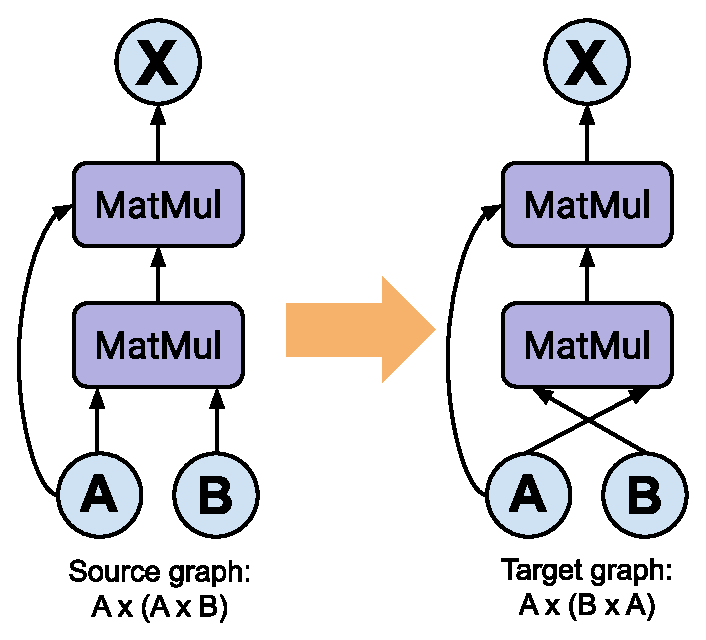
\includegraphics[height=3cm]{sections/3problem/images/rewrite1}%
      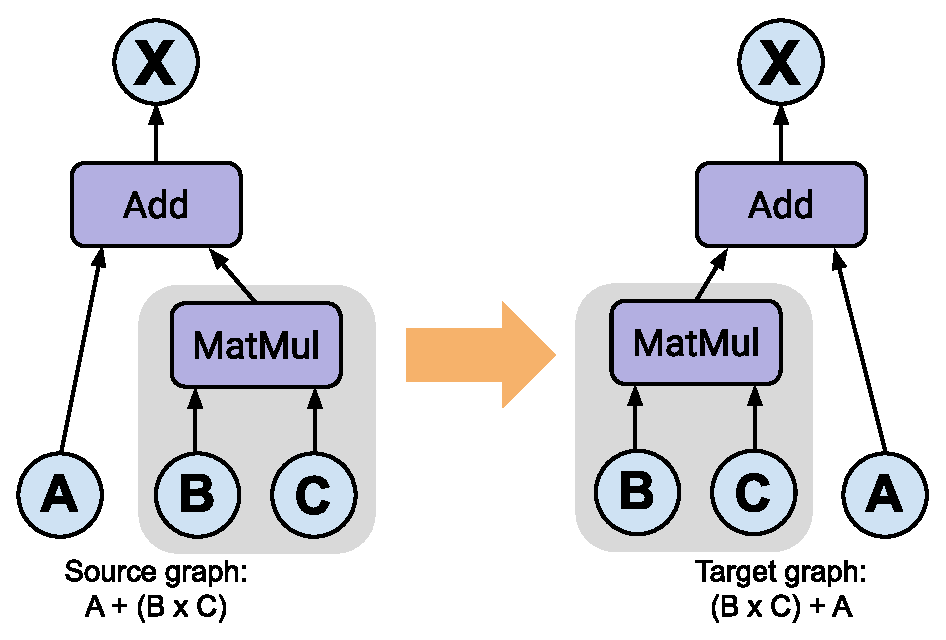
\includegraphics[height=3cm]{sections/3problem/images/rewrite2}%
    }%
  }
  \setlength{\twosubht}{\ht\twosubbox}
  
  % typeset
  \centering
  \subcaptionbox{Tensor renaming substitution \label{fig:problem:rewrite-graph1}}{
    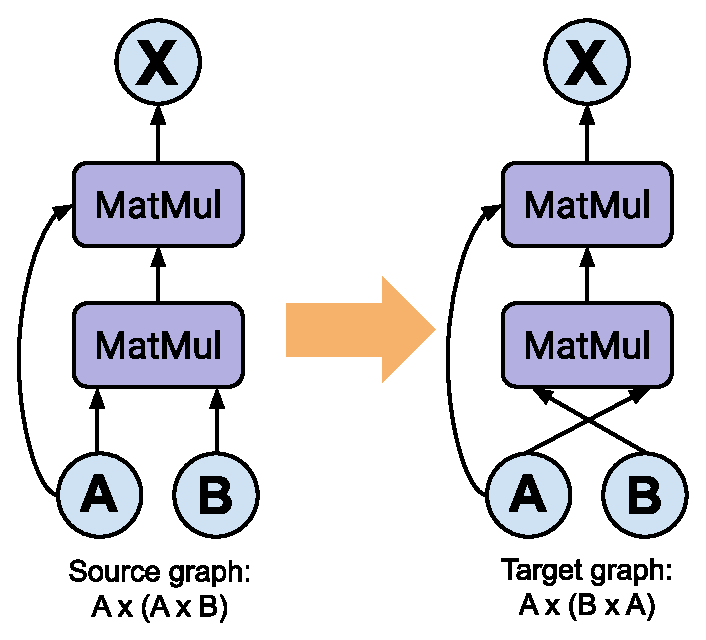
\includegraphics[height=\twosubht]{sections/3problem/images/rewrite1}
  }\quad
  \subcaptionbox{Common subgraph substitution \label{fig:problem:rewrite-graph2}}{
    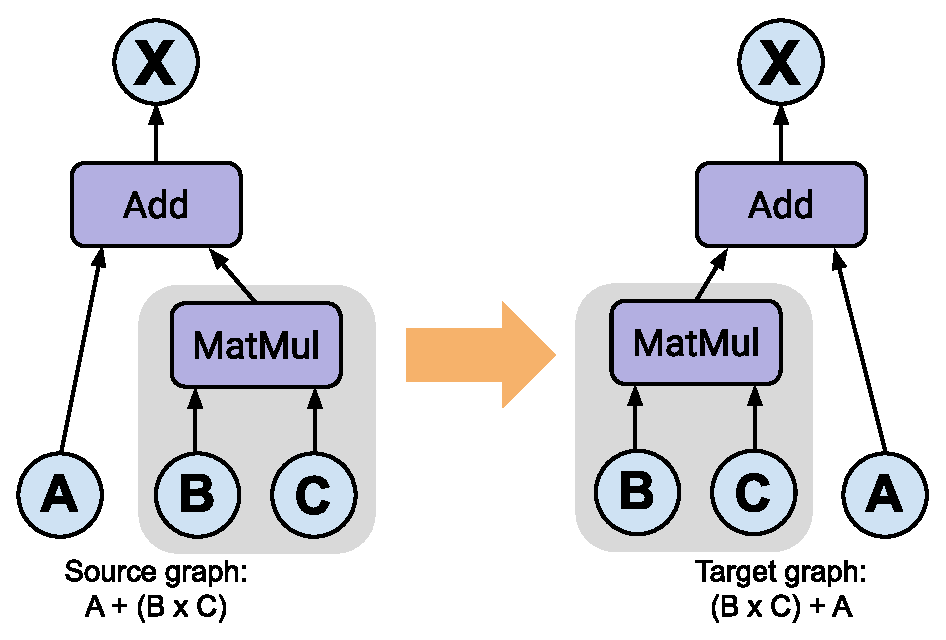
\includegraphics[height=\twosubht]{sections/3problem/images/rewrite2}
  }
  \caption[Two examples of trivial graph substitutions]{Two examples of trivial graph substitutions that does not impact the overall runtime of the computation graph. The left sub-figure shows a simple renaming of the tensor inputs. The figure on the right shows that we have a common sub-graph between the source and the target graphs. In both cases we eliminate the duplicates as the hash of the two graphs will be identical.}
\end{figure}

In this work, we take the same approach as that of TASO and automatically generate the candidate graphs. We perform this as an offline step as it requires a large amount of computation to both generate and verify the candidate substitution; to place an upper bound on the computation, we limit the input tensor size to a maximum of 4x4x4x4 during the verification process. Following the generation and verification steps, we prune the collection to remove substitutions that are considered trivial and as such would not impact runtime. For example, trivial substitutions include input tensor renaming and common subgraphs, we show both techniques diagrammatically in Figure \ref{fig:problem:rewrite-graph1} and \ref{fig:problem:rewrite-graph2} respectively.

\subsection{Graph Embedding}
\label{sec:design:subsec:embed}
% As we described in the previous section, the reinforcement learning agent must learn to choose two actions at each step in an epoch; the transformation and location from the set available dependent on the current computation graph. To learn the optimal action selection, we must create an embedding from the computation graph representation in the machine learning framework to our internal, manipulable graph representation inside our environment, our modified TASO backend.

When developing the project, a pivotal part of the project is the decision as the representation of the GNN as there are a wide variety of forms which it can take. For example, a common implementation are message-passing networks (MPNNs) \cite{gilmer2017neural} which reduce data along edges and between nodes in the graph. Alternatively, we considered using graph convolutional networks (GCNs) \cite{kipf2016semi}, however, we found that using messages passing networks produced a more generalisable embedding as we leverage the relational biases in the graph structure and avoid imposing restrictions on the learned embedding accidentally.

[TODO] cite related work that used GNNs in Computer Systems

During training of the reinforcement learning agents, we convert the internal graph representation to a graph neural network. In order to train the model-free and model-based agents, a latent space embedding of the computation graph is required. Therefore, using the \texttt{graph\textunderscore nets} package developed by Battaglia et al. \cite{battaglia2018relational}, we use the graph neural network to learn a latent space embedding of the graph using message passing networks to gather the global learned features of the graph.

[TODO also describe the embedding parameters for graph network]

Furthermore, we acknowledge the work by Kai Fricke and Michael Schaarschmidt who developed the initial Python interface with TASO, the algorithm for converting the C++ TASO graph representation into a Cython object and performed experiments a model-free reinforcement learning agent \cite{xflowrl2019}. We used their work as a foundation upon which we continued development and research into model-free and model-based RL.


\section{Reinforcement Learning formulation}
In the following section we will describe how to represent the computation graph optimisation problem in the reinforcement learning domain by describing the key components of the system. We describe the system environment in which the agents act, the state-action space, and finally the reward functions for both the model-free and model-based agents which we used to determine the optimal reward signal to train the agents.

\subsection{System environment}
\label{sec:prob:subsec:sysenv}

In order to train a reinforcement learning agent, it necessary that we have access to an environment that, given the current environment state, the agent can take an action. After taking the chosen action, the environment is updated into a new state and the agent receives a reward signal. Typically, one uses a mature environment such as OpenAI Gym \cite{brockman2016openai} or OpenSpiel \cite{LanctotEtAl2019OpenSpiel} as the quality of the environment often has a significant effect on the stability of training. Moreover, using an environment that uses a common interface allows researchers to implement algorithms with ease and, importantly, reproduce results from published conference papers.

In our work, we implemented an environment that follows the OpenAI Gym API standard stepping an environment, that is, we have a function \texttt{step(action)} that accepts a single parameter, the action requested by the agent to be performed in the environment. The \texttt{step} function returns a 4-tuple \texttt{(next\textunderscore state, reward, terminal, extra\textunderscore info)}. \texttt{extra\textunderscore info} is a dictionary which can store arbitrary data. The environment in our project has a structure that is shown diagrammatically in figure \ref{fig:problem:sys-env}.

\begin{figure}[ht]
  \centering
  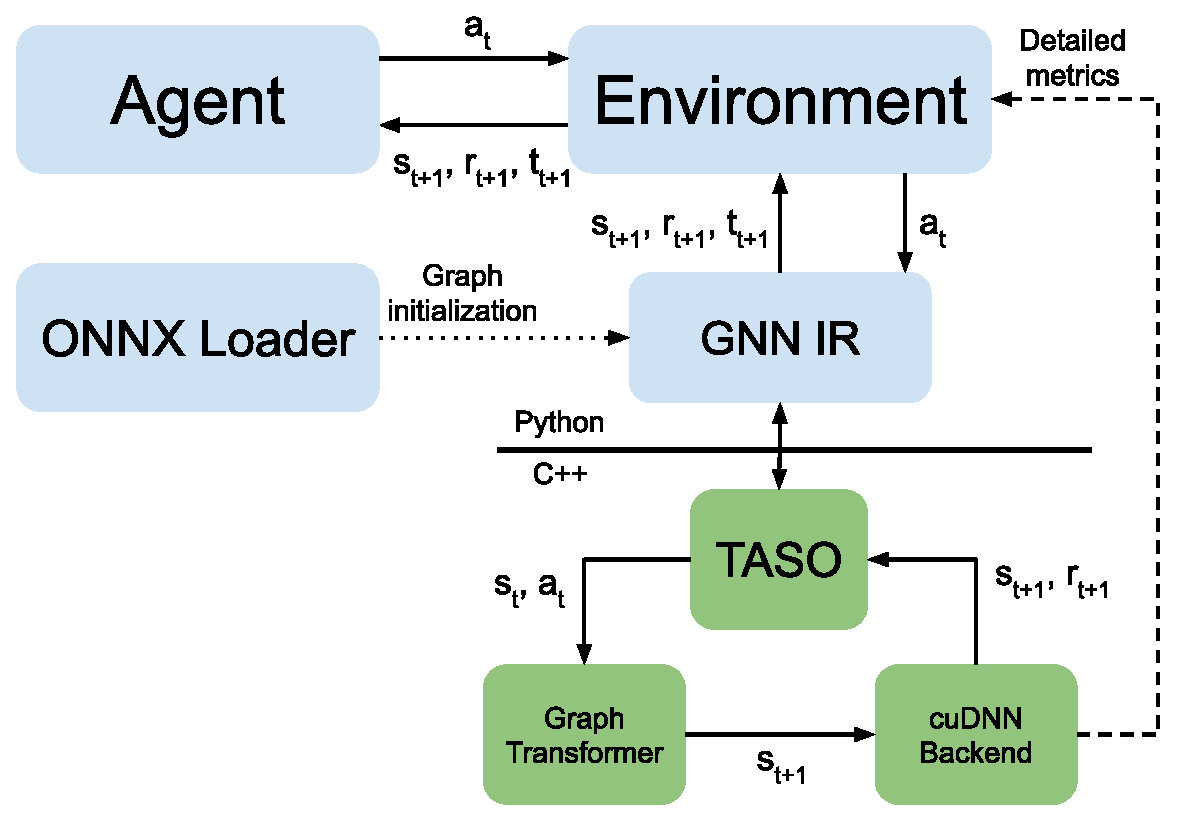
\includegraphics[width=0.75\columnwidth]{sections/3problem/images/sysenv}
  \caption[RL system environment]{Data flow between components of the RL system. Although this diagram shows the setup for both the training of the model-free and model-based world model, we can use the environment in figure \ref{fig:bg:mb-rl} as a drop-in replacement of the environment to train the model-based controller.}
  \label{fig:problem:sys-env}
\end{figure}

To simplify the implementation of the environment, we used made extensive use of the work by Jia et al. \cite{jia2019taso} with the open source version of TASO. We provide a computation graph and the chosen transformation and location; TASO then applies the requested transformation and returns the newly transformed graph. Further, we use internal TASO functions that calculates estimates of the runtime on the hardware device which we use as our reward signal for training the agent. During our experiments we modified TASO to extract detailed runtime measurements to analyse the rewards using a range of different reward formulae---we provide more detail in section \ref{sec:prob:subsec:rwd}.

The scope of our work meant that there was no existing prior work that applied reinforcement learning to the task of optimising deep learning computation graphs. Thus, we required an environment in which an agent can act efficiently. Due to the nature of systems environments, the interactions with the real-world environment can be often slow, especially compared to those such as Arcade Learning Environment \cite{Bellemare_2013}. An aim of this work was to train a simulated environment, a ``world model'', that if accurate in relation to the real environment, we can train an agent far more efficiently than would be possible with the real-environment. In sections \ref{sec:rlopt:subsec:mb-agent} and \ref{sec:eval:subsec:mbagent} we will further explore world models and evaluate our implementation respectively.

\subsection{Computation Graphs}
The first step prior to optimising a deep learning graph is that we must load, or create on-demand, the model in a supported deep learning framework. In our project, we can support any model that is serialised into the ONNX \cite{bai2019onnx} format which is a open-source standard for defining the structure of deep learning models. Thereby, by extension, we can support any deep learning framework that supports ONNX serialisation such as TensorFlow \cite{tensorflow2015-whitepaper}, PyTorch \cite{pytorch} and MXNet \cite{chen2015mxnet}.

Next, we parse the ONNX graph internal representation by converting all operators into the equivalent TASO tensor representations such that we can modify the graph using the environment API as we described in section \ref{sec:prob:subsec:sysenv}. Although our environment does not support conversion of all operators defined in the ONNX specification \footnote{ONNX operator specification:~\url{https://github.com/onnx/onnx/blob/master/docs/Operators.md}}, the majority of the most common operators for our use case are supported; therefore we still maintain the semantic meaning and structure of the graph. Additionally, after performing optimisations of the graph, we can export the optimised graph directly to an ONNX format.

\subsection{State-Action space}
\label{sec:prob:subsec:sap}
In this project we modelled the state and action space in accordance with prior research, specifically we referenced work in a similar domain of system optimisation using reinforcement learning; Mirhoseini et al. \cite{mirhoseini2018hierarchical} used hierarchical RL with multiple actions to find the optimal device placement and Addanki et al. \cite{addanki2019placeto} that also aided in the design choice of input/output graph sizes.

Next, we require two values in order to update the environment. First, we need a select a transformation (which we refer to as an \texttt{xfer}) to apply to the graph. Secondly, the location at which to apply the transformation. As we need to select two actions that are dependent on each other to achieve a higher performance, it requires selecting the actions simultaneously.

However, this would require a model output of $N \times L$ values, where $N$ is the number of transformations, $L$ is the number of locations. Such an action space is too large to train a model to efficiently predict the correct action. Additionally, after choosing a transformation, we ideally mask the available locations as not all locations can be used to apply a transformation. Therefore, using the same trunk network, we first predict the transformation, apply the location mask for the selected transformation, then predict the location.

We define the action as 2-value tuple of (xfer\textunderscore id, location). There is a special case for the xfer\textunderscore id. When it equals N (the number of available transformations), we consider it the NO-OP action. Therefore, in this special case we do not modify the graph, rather we terminate the current episode and reset the environment to its initial state.

As explained in the previous section, we used an step-wise approach where at each iteration, we provide a 2-tuple of the transformation and location, to apply in the current state. The updated state from the environment is a 4-tuple consisting of \texttt{(graph\textunderscore tuple, xfer\textunderscore tuples, location\textunderscore masks, xfer\textunderscore mask)}.

\texttt{xfer\textunderscore mask} refers to a binary mask that indicates the valid and invalid transformations that can be applied to the current computation graph as not every transformation can be applied to every graph. If the current graph has only four possible transformations that can be applied, all other transformations considered to be invalid. Thus, we return a boolean location mask where only valid transformations are set to 1, or \texttt{true}. This can be used to zero-out the model logits of invalid transformations (and thereby actions also) to make ensure the agent always selects a valid transformation from the set.

Similarly, for each transformation selected by the agent, there are a number of valid locations where this transformation can be applied. We set a hardcoded, albeit configurable, limit the number of locations to 200 in this work. If the current graph has fewer than 200 possible locations for any given transformation, the remaining are considered invalid. Therefore, we again return a boolean location mask, which is named \texttt{location\textunderscore masks} in the 4-tuple defined above, which can be used to zero out the model logits that which the locations are invalid. 

% We use the location masks for every transformation, therefore, we have a $N \times L$ tensor, where $N$ is the number of transformations, and $L$ is the maximum number of valid locations.

\subsection{Reward function}
\label{sec:prob:subsec:rwd}

We further note that TASO used a simple method to estimate the runtime of tensor operators that are executed using low-level CUDA APIs and the runtime is averaged over $N$ forward passes. However, this approach to runtime estimation is imperfect as there is a non-negligible variance of the runtime on real hardware. We investigated the use of using real runtime measurements during training rather than a estimation of operator runtime. We found that it increases duration of each training step such that performance improvements are not worth the trade-off.

- Runtime difference

- Inclusion of detailed measurements

- Real-time measurements instead of estimated

% - Look up research on RL rewards (what makes a good reward signal)